\documentclass[aspectratio=169]{beamer}

% ---------------------------------------------------------------------------
% Theme
% ---------------------------------------------------------------------------
\usetheme{Boadilla}
\usecolortheme{seahorse}
\setbeamertemplate{navigation symbols}{}
\setbeamertemplate{footline}[frame number]
\setbeamerfont{frametitle}{size=\large,series=\bfseries}

\usepackage{tikz}
\usetikzlibrary{arrows.meta, positioning, fit, backgrounds, calc}
\usepackage{amsmath}
\usepackage{amssymb} % \checkmark
\usepackage{booktabs}
\usepackage{xcolor}

% Palette
\definecolor{cEnc}{RGB}{52,120,184}
\definecolor{cDyn}{RGB}{200,120,40}
\definecolor{cDec}{RGB}{70,160,90}
\definecolor{cAct}{RGB}{170,60,150}
\definecolor{cBad}{RGB}{200,50,50}
\definecolor{cGood}{RGB}{40,150,70}

\newcommand{\good}[1]{\textcolor{cGood}{#1}}
\newcommand{\bad}[1]{\textcolor{cBad}{#1}}

\title[Atari Breakout World Model]{Learning an Action-Conditioned World Model\\for Atari Breakout}
\subtitle{Milestone 2 --- Technical Approach}
\author{}
\date{May 22, 2026}

\begin{document}

% ---------------------------------------------------------------------------
\begin{frame}
  \titlepage
\end{frame}

% ---------------------------------------------------------------------------
\begin{frame}{Goal: a learned simulator of the game}
  \begin{columns}
    \begin{column}{0.58\textwidth}
      \textbf{A world model} predicts how the game evolves --- given past
      frames and an action, generate the next frame.

      \vspace{0.5em}
      \textbf{Our target:} feed a few start frames + an action sequence, then
      \emph{roll out} a playable-looking clip:
      \begin{itemize}
        \item paddle moves with the action
        \item ball bounces off paddle and walls
        \item bricks break on contact
      \end{itemize}

      \vspace{0.5em}
      \textbf{Why it's hard:} the ball is 1--2 pixels at $64\times64$; tiny
      errors compound during autoregressive rollout.
    \end{column}
    \begin{column}{0.42\textwidth}
      \centering
      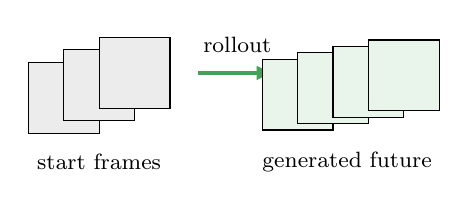
\begin{tikzpicture}[scale=0.9]
        \foreach \i/\x in {0/0, 1/0.5, 2/1.0} {
          \node[draw, fill=gray!15, minimum size=0.9cm] at (\x,\x*0.35) {};
        }
        \node at (0.5,-0.9) {\footnotesize start frames};
        \draw[-{Latex[length=2.5mm]}, very thick, cDec]
          (1.9,0.35) -- (3.0,0.35);
        \node at (2.45,0.75) {\footnotesize rollout};
        \foreach \i/\x in {0/3.3, 1/3.8, 2/4.3, 3/4.8} {
          \node[draw, fill=cDec!12, minimum size=0.9cm] at (\x,\x*0.18-0.55) {};
        }
        \node at (4.0,-0.9) {\footnotesize generated future};
      \end{tikzpicture}
    \end{column}
  \end{columns}
\end{frame}

% ---------------------------------------------------------------------------
\begin{frame}{Task \& Data}
  \begin{columns}
    \begin{column}{0.55\textwidth}
      \textbf{Environment:} Atari Breakout via the Arcade Learning Environment.

      \vspace{0.4em}
      \textbf{Observations:} $64\times64$ grayscale frames.

      \vspace{0.4em}
      \textbf{State:} a stack of the last \textbf{4 frames} (gives velocity).

      \vspace{0.4em}
      \textbf{Actions:} 4 discrete actions (one-hot), collected with random play.

      \vspace{0.4em}
      \textbf{Sequences:} length-20 trajectories; thousands of them.
    \end{column}
    \begin{column}{0.45\textwidth}
      \textbf{How we use it}
      \begin{itemize}
        \item \textbf{Train:} predict frame $t{+}1$ from frames $[t{-}3..t]$ and
              action $a_t$.
        \item \textbf{Teacher-forced} eval: every input is a \emph{real} frame
              $\Rightarrow$ isolates one-step quality.
        \item \textbf{Rollout} eval: feed the model its \emph{own} predictions
              $\Rightarrow$ tests long-horizon stability.
      \end{itemize}
    \end{column}
  \end{columns}
\end{frame}

% ---------------------------------------------------------------------------
\begin{frame}{Method: FiLM-Action U-Net World Model}
  \centering
  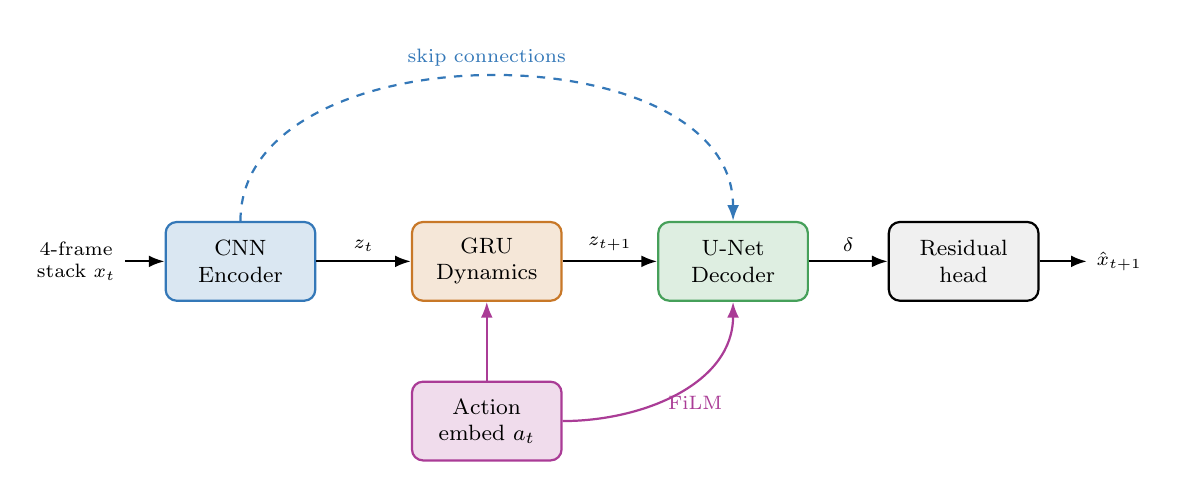
\begin{tikzpicture}[
      box/.style={draw, rounded corners, minimum height=1.0cm, minimum width=1.9cm,
                  align=center, font=\footnotesize, thick},
      sm/.style={font=\scriptsize},
      ar/.style={-{Latex[length=2mm]}, thick}
    ]
    \node[box, fill=cEnc!18, draw=cEnc] (enc) at (0,0) {CNN\\Encoder};
    \node[box, fill=cDyn!18, draw=cDyn, right=1.2cm of enc] (dyn) {GRU\\Dynamics};
    \node[box, fill=cDec!18, draw=cDec, right=1.2cm of dyn] (dec) {U-Net\\Decoder};
    \node[box, fill=gray!12, right=1.0cm of dec] (head) {Residual\\head};

    \node[sm, left=0.5cm of enc, align=center] (in) {4-frame\\stack $x_t$};
    \node[sm, right=0.6cm of head, align=center] (out) {$\hat{x}_{t+1}$};

    \draw[ar] (in) -- (enc);
    \draw[ar] (enc) -- node[sm, above]{$z_t$} (dyn);
    \draw[ar] (dyn) -- node[sm, above]{$z_{t+1}$} (dec);
    \draw[ar] (dec) -- node[sm, above]{$\delta$} (head);
    \draw[ar] (head) -- (out);

    % action
    \node[box, fill=cAct!18, draw=cAct, below=1.0cm of dyn] (act) {Action\\embed $a_t$};
    \draw[ar, cAct] (act) -- (dyn);
    \draw[ar, cAct] (act) to[out=0,in=-90] node[sm, right, pos=0.4]{FiLM} (dec.south);

    % skip connections
    \draw[ar, cEnc, dashed] (enc.north) to[out=90,in=90]
        node[sm, above, pos=0.5]{skip connections} (dec.north);
  \end{tikzpicture}

  \vspace{0.6em}
  \footnotesize
  \[
    z_t = \mathrm{Enc}(x_t),\quad
    z_{t+1} = \mathrm{GRU}([z_t, e(a_t)]),\quad
    \hat{x}_{t+1} = \mathrm{clamp}\big(x_t^{\text{last}} + s\cdot\tanh(\delta),\,0,1\big)
  \]
\end{frame}

% ---------------------------------------------------------------------------
\begin{frame}{Design intuition --- three choices, three fixed failures}
  We arrived at each component by \emph{diagnosing a concrete failure}:

  \vspace{0.6em}
  \begin{enumerate}
    \item \textbf{U-Net skip connections} \\
      \bad{Failure:} a 256-d global latent cannot encode a 1-pixel ball location
      $\Rightarrow$ blurry, fading ball. \\
      \good{Fix:} skips pipe pixel detail straight to the decoder.

    \vspace{0.4em}
    \item \textbf{FiLM action conditioning} \\
      \bad{Failure:} a 4-d action concatenated to a 256-d latent is $<2\%$ of the
      signal $\Rightarrow$ \emph{action ignored} (sensitivity exactly $0.000$). \\
      \good{Fix:} action modulates every decoder feature map; cannot be optimized away.

    \vspace{0.4em}
    \item \textbf{Bounded residual decoder} \\
      \bad{Failure:} free pixel output collapses to the mean ``brick-wall'' frame. \\
      \good{Fix:} predict a small bounded \emph{change} to the previous frame.
  \end{enumerate}
\end{frame}

% ---------------------------------------------------------------------------
\begin{frame}{Why we expect this to work}
  \begin{columns}
    \begin{column}{0.5\textwidth}
      \textbf{Key insight}

      One-step Breakout is \emph{nearly deterministic}: given the true 4-frame
      stack + action, the next frame is essentially fixed.

      \vspace{0.4em}
      So an L1-trained model \emph{can} fit it sharply --- the classic
      ``L1 = blur'' problem only bites under genuine multi-modal uncertainty
      (i.e.\ long rollout), not one-step.

      \vspace{0.4em}
      \textbf{Loss} (motion-aware):
      \[
        \mathcal{L} = \underbrace{w\!\cdot\!\text{L1}}_{\text{image}}
        + \lambda_1 \underbrace{\Delta\text{-loss}}_{\text{changed px}}
        + \lambda_2 \underbrace{\text{false-motion}}_{\text{still px}}
      \]
    \end{column}
    \begin{column}{0.5\textwidth}
      \textbf{Decompose the problem}
      \begin{itemize}
        \item \textbf{Encoder + skips} $\to$ \emph{what} is on screen
        \item \textbf{GRU + action} $\to$ \emph{where} things move
        \item \textbf{Residual head} $\to$ \emph{small edits}, not repaint
      \end{itemize}

      \vspace{0.6em}
      Each module has one job, so failures are \emph{diagnosable} --- which is how
      we debugged the three issues on the left.
    \end{column}
  \end{columns}
\end{frame}

% ---------------------------------------------------------------------------
\begin{frame}{Baselines}
  \centering
  \renewcommand{\arraystretch}{1.3}
  \begin{tabular}{lll}
    \toprule
    \textbf{Baseline} & \textbf{What it tests} & \textbf{Expected weakness} \\
    \midrule
    Copy-last-frame & lower bound; ball moves $\sim$1 px & no motion at all \\
    Bottleneck (no skips) & value of skip connections & blurry / fading ball \\
    Concat-action (no FiLM) & value of FiLM & ignores the action \\
    Residual, no rollout train & one-step vs rollout gap & rollout collapses \\
    \midrule
    \textbf{Ours} (FiLM U-Net + rollout) & full method & --- \\
    \bottomrule
  \end{tabular}

  \vspace{0.8em}
  \footnotesize
  Each baseline is an \textbf{ablation} of one design choice --- so the comparison
  directly measures what each component buys us.
\end{frame}

% ---------------------------------------------------------------------------
\begin{frame}{Experimental setup \& evaluation}
  \begin{columns}
    \begin{column}{0.48\textwidth}
      \textbf{Setup}
      \begin{itemize}
        \item Optimizer: AdamW, lr $10^{-4}$
        \item Train teacher-forced first; then add an autoregressive
              \textbf{rollout loss} (curriculum: warmup $\to$ ramp)
        \item Compute: MPS / Colab GPU for full runs
      \end{itemize}

      \vspace{0.5em}
      \textbf{Metrics}
      \begin{itemize}
        \item One-step error (teacher-forced)
        \item \textbf{Rollout coherence horizon}: \#frames before motion collapses
        \item \textbf{Action sensitivity}: $\|\hat{x}(a_i)-\hat{x}(a_j)\|$
        \item Physics check: ball-centroid trajectory
      \end{itemize}
    \end{column}
    \begin{column}{0.52\textwidth}
      \centering
      \textbf{Diagnostic tooling we built}
      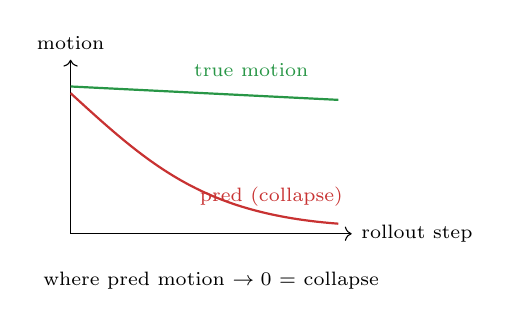
\begin{tikzpicture}[scale=0.85, every node/.style={font=\scriptsize}]
        \draw[->] (0,0) -- (4.2,0) node[right]{rollout step};
        \draw[->] (0,0) -- (0,2.6) node[above]{motion};
        \draw[thick, cGood] (0,2.2) -- (4,2.0) node[right, black]{};
        \node[cGood] at (2.7,2.45) {true motion};
        \draw[thick, cBad] (0,2.1) .. controls (1.2,1.0) and (2,0.3) .. (4,0.15);
        \node[cBad] at (3.0,0.55) {pred (collapse)};
        \node at (2.1,-0.7) {\scriptsize where pred motion $\to 0$ = collapse};
      \end{tikzpicture}
    \end{column}
  \end{columns}
\end{frame}

% ---------------------------------------------------------------------------
\begin{frame}{Current progress}
  \begin{columns}
    \begin{column}{0.55\textwidth}
      \textbf{Done}
      \begin{itemize}
        \item[\good{\checkmark}] Data pipeline (ALE $\to$ sequences + actions)
        \item[\good{\checkmark}] FiLM-action U-Net implemented
        \item[\good{\checkmark}] \textbf{Clean one-step teacher-forced prediction} ---
              visible ball \emph{and} paddle, correct motion, no noise
        \item[\good{\checkmark}] Action sensitivity: $0.000 \to$ nonzero (FiLM works)
        \item[\good{\checkmark}] Diagnostic suite (sensitivity, motion trace, GIFs)
      \end{itemize}

      \textbf{Next}
      \begin{itemize}
        \item[$\rightarrow$] Rollout training + measure coherence horizon
        \item[$\rightarrow$] Run ablations (the baselines)
        \item[$\rightarrow$] Stretch: discrete-token model (IRIS-style) for
              long-horizon sharpness
      \end{itemize}
    \end{column}
    \begin{column}{0.45\textwidth}
      \centering
      \footnotesize
      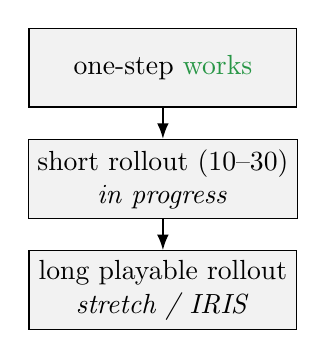
\begin{tikzpicture}
        \node[draw, fill=gray!10, minimum width=3.4cm, minimum height=1.0cm, align=center]
          (a) {one-step \good{works}};
        \node[draw, fill=gray!10, minimum width=3.4cm, minimum height=1.0cm, align=center,
          below=0.4cm of a] (b) {short rollout (10--30) \\ \emph{in progress}};
        \node[draw, fill=gray!10, minimum width=3.4cm, minimum height=1.0cm, align=center,
          below=0.4cm of b] (c) {long playable rollout \\ \emph{stretch / IRIS}};
        \draw[-{Latex[length=2mm]}, thick] (a) -- (b);
        \draw[-{Latex[length=2mm]}, thick] (b) -- (c);
      \end{tikzpicture}
    \end{column}
  \end{columns}
\end{frame}

% ---------------------------------------------------------------------------
\begin{frame}{Summary}
  \begin{itemize}
    \item \textbf{Goal:} action-conditioned world model that rolls out
          game-like Breakout clips.
    \item \textbf{Method:} FiLM-action U-Net --- skips for detail, FiLM for action,
          bounded residual for stable edits.
    \item \textbf{Each design choice fixes a measured failure} (blur,
          action-ignored, mode collapse).
    \item \textbf{Status:} one-step prediction is clean; rollout training and
          ablations are next.
    \item \textbf{Evaluation centers on the rollout coherence horizon} --- the
          honest measure of a world model.
  \end{itemize}
  \vspace{0.6em}
  \centering
  \large Thank you --- questions?
\end{frame}

\end{document}
